\section{Results}

\subsection{Case study}
With the tools developed it is possible to study a wide variety of flight situations. To keep the study consice we will limit our analysis to the situation of engine failure at take off with landing gear retracted as described by CS25.121, CS25.147 and CS12.149 \cite{CS25}. Although refering to a single certification rule, the ensight given on the tool efficiency to compare aircraft configuration and potential of differential thrust is well demonstrated.

The certification rules indicate different flight conditions for twin engine and more than four engines. The main differences are resumed in table %CS25.121 states the following flight conditions:
\begin{table}[hbt]
	\caption{\label{tab:DiffTwinMulti} Certification differences between twin-engines and more than four engines, \cite{CS25}} 
	\centering
	\begin{tabular}{l|l|c}
		Parameters & Twin engine & More than four engines\\
		\hline
		Gradient of climb, critical engine inoperative & $\leq 2.4\%$ & $\leq 3.0\%$\\
		Heading change of $15\degree$ at 1.3$V_{SR_1}$& One engine inoperational & Two critical engines inoperational\\
		$V_{MC} < 1.13 V_{SR}$ & One engine inoperative & One critical engine inoperative \\
	\end{tabular}
\end{table}

\begin{table}[hbt]
	\caption{\label{tab:ConfigurationStudied} Configuration studied}
	\centering
	\begin{tabular}{l|c|c|c}
		Parameters & Original ATR72 & DEP ATR72 & DEP ATR72 with small VT\\
		\hline
		Engines & 2 & 12 & 12\\
		Inoperative engines & 1 & 3 & 3\\
		VT area & $S_{v_0}$ & $S_{v_0}$ & $0.7 S_{v_0}$\\
		Gradient of climb & $3.0\%$ & $3.0\%$ & $3.0\%$\\
		Rudder allowed & Yes & No & No\\
		\hline
		Additional Parameters & & & \\
		\hline
		$V_{\textrm{app}}$=$1.13V_{\textrm{app}}$ (m/s)& 56 & 56 & 56\\
		$V_{\textrm{sr}}$ (m/s)& 50.5 & 50.5 & 50.5\\
		$1.3V_{\textrm{sr}}$ (m/s)& 65 & 65 & 65\\
		VT stall limit & $\beta=15\degree$ & $\beta=15\degree$ & $\beta=15\degree$\\
	\end{tabular}
\end{table}

%\begin{itemize}
%\item Climb gradient with one engine inoperative may not be less than 2.4\% for twin engines
%\item Climb gradient with one engine inoperative may not be less than 3\% for aircrafts with four engines or more.
%\end{itemize}

\begin{figure}[hbt!]
	\centering
	\begin{subfigure}{0.49\textwidth}
		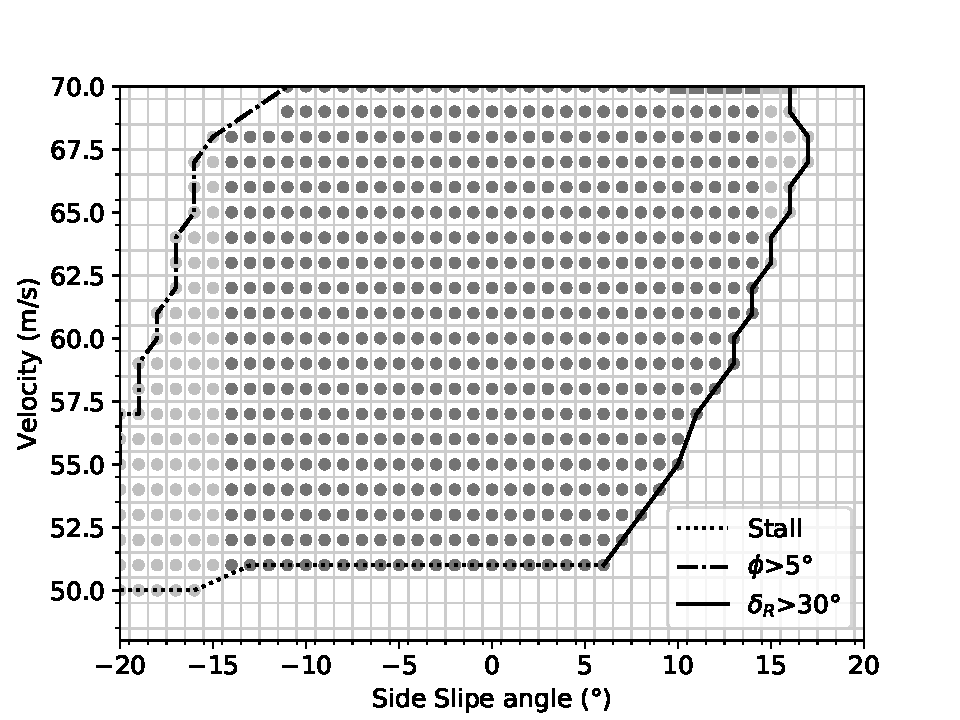
\includegraphics[width=0.95\textwidth]{originalMapBetaVelfin1Eng3RudFalse}
		\caption{Original ATR72 with one engine failure.}
		\label{fig:originalfin1_3engine}
	\end{subfigure}
	\begin{subfigure}{0.49\textwidth}
		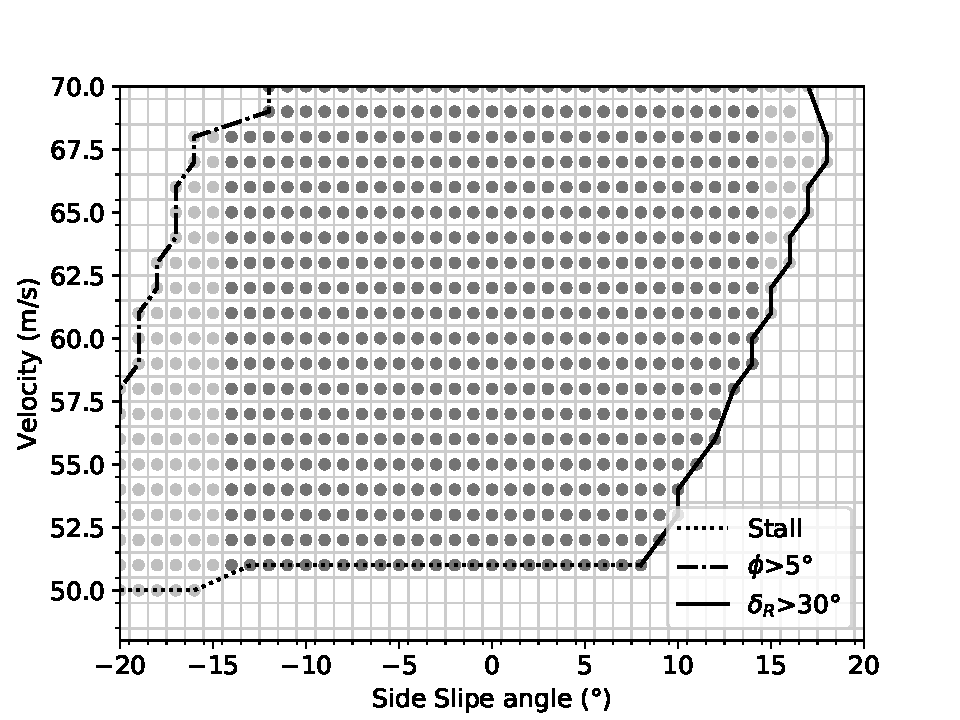
\includegraphics[width=0.95\textwidth]{originalMapBetaVelfin1Eng15RudFalse}
		\caption{ATR with 12 engines, three inoperatives.}
		\label{fig:originalfin1_15engine}
	\end{subfigure}
	\caption{Original ATR with \ref{fig:originalfin1_3engine} twin engine, one inoperational and \ref{fig:originalfin1_15engine} twelve engines, three inoperationals. Only the rudder is used to compensate the yawing moment.}
\end{figure}

\begin{figure}
	\begin{subfigure}{0.49\textwidth}
		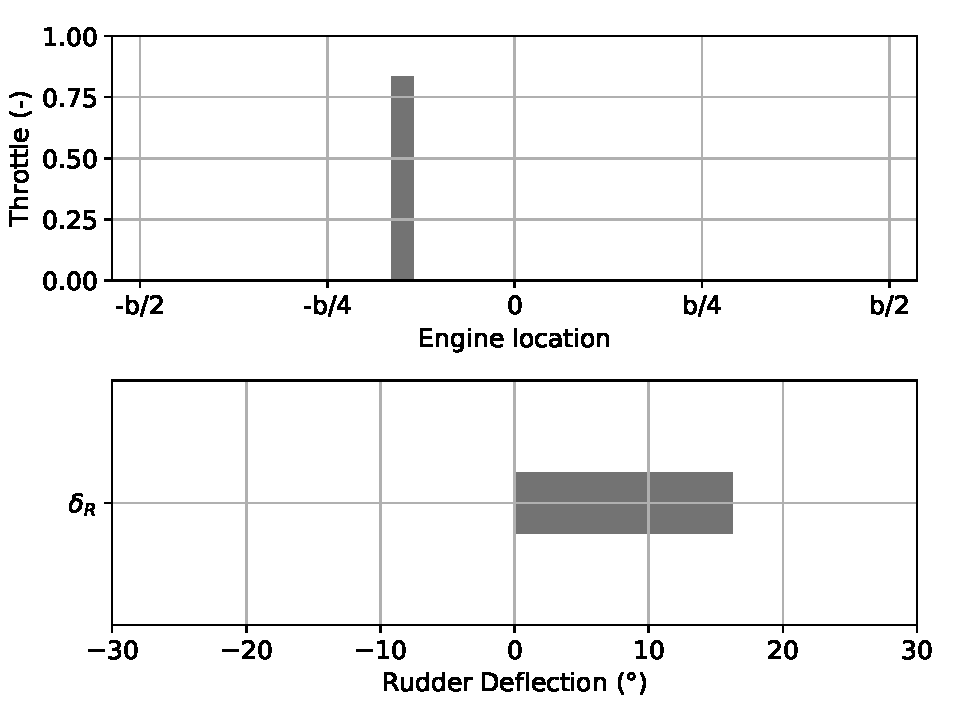
\includegraphics[width=0.95\textwidth]{Defloriginalfin1Eng3RudFalse}
		\caption{Original ATR72 with one engine failure.}
		\label{fig:Defloriginalfin1_3engine}
	\end{subfigure}
	\begin{subfigure}{0.49\textwidth}
		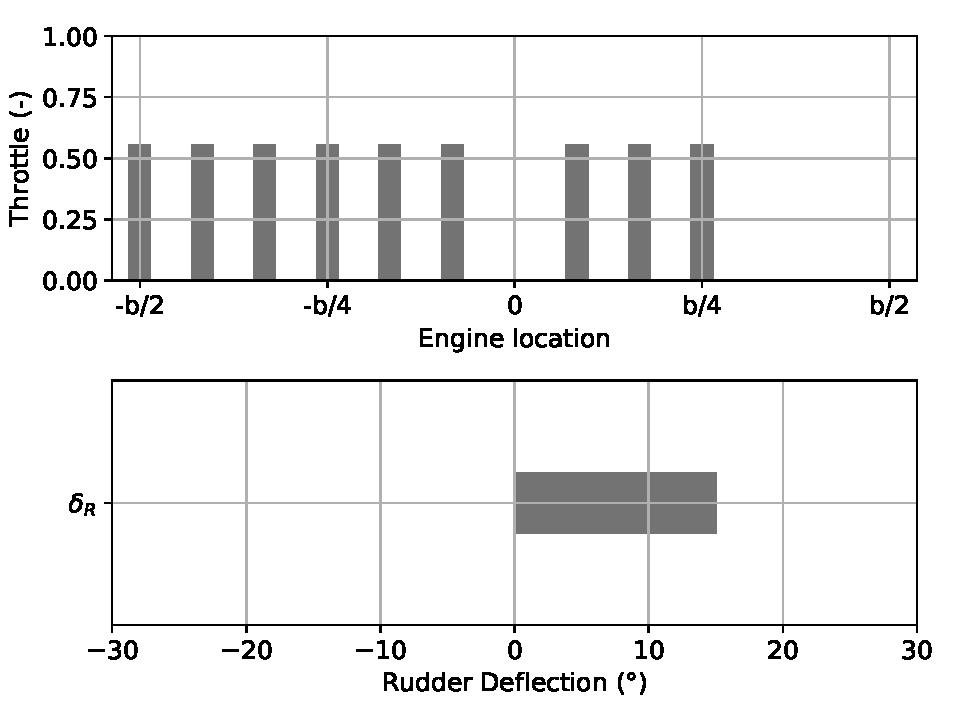
\includegraphics[width=0.95\textwidth]{Defloriginalfin1Eng15RudFalse}
		\caption{Original ATR with twelve engines, three inoperatives.}
		\label{fig:Defloriginalfin1_15engine}
	\end{subfigure}
	\caption{Throttle level and rudder deflection for trim at V=60m/s, $\beta=0$}
\end{figure}

\begin{figure}[hbt!]
		\centering
		\begin{subfigure}{0.49\textwidth}
			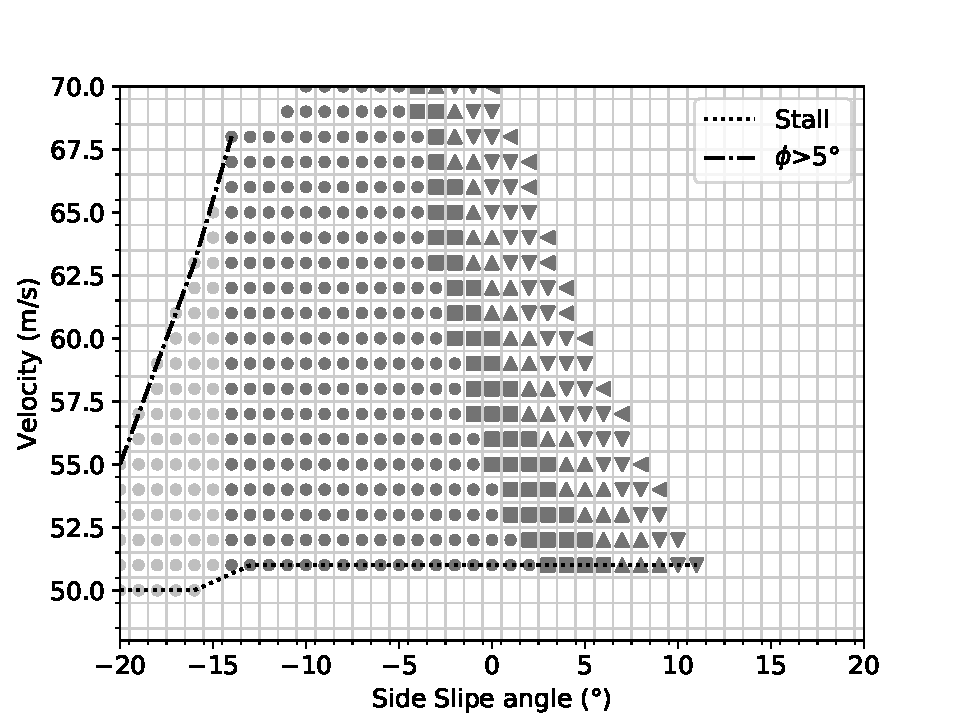
\includegraphics[width=0.95\textwidth]{DEPoriginalMapBetaVelfin1Eng15RudTrue}
			\caption{Flight envelop, ATR with 12 engines, three inoperatives.}
			\label{fig:DEPoriginalfin1_15engine}
		\end{subfigure}
		\begin{subfigure}{0.49\textwidth}
			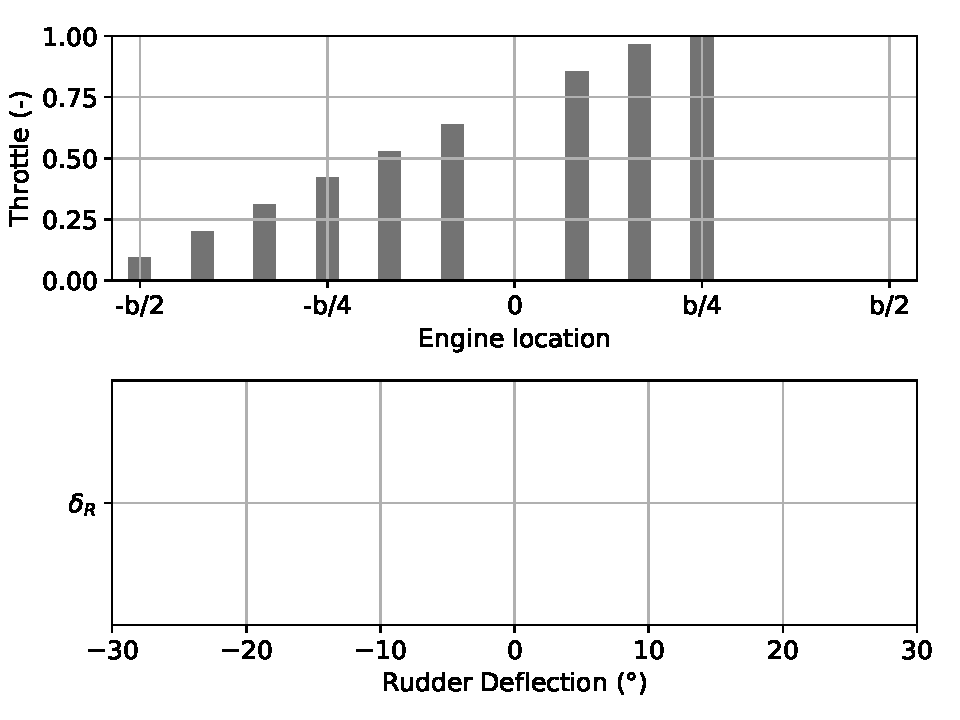
\includegraphics[width=0.95\textwidth]{DeflDEPoriginalfin1Eng15RudTrue}
			\caption{Throttle level and Rudder deflection at 60m/s and $\beta=0\degree$, ATR72 with 12 engines, three inoperatives.}
			\label{fig:DeflDEPoriginalfin1_15Eng}
		\end{subfigure}
		\caption{ATR72 using only differential thrust. Circles indicate an equilibrium point, rectangle indicate an equilibrium with at least one engine at saturation (full throttle)}
\end{figure}

\begin{figure}[hbt!]
	\centering
	\begin{subfigure}{0.49\textwidth}
		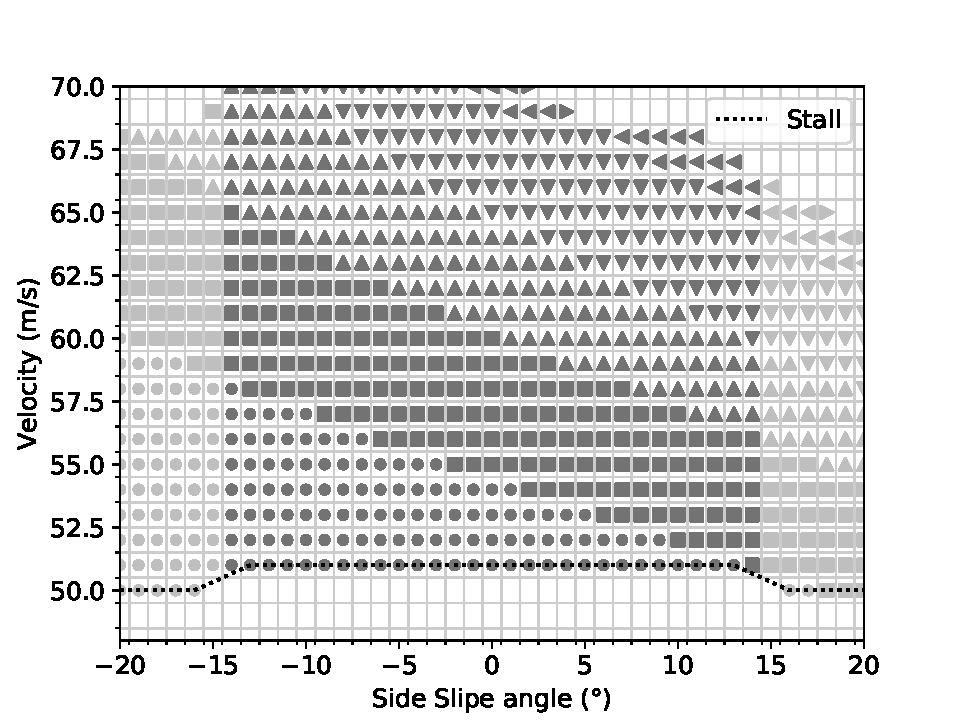
\includegraphics[width=0.95\textwidth]{DEPoriginalMapBetaVelfin07Eng15RudTrue}
		\caption{ATR with 12 engines, three inoperatives and $S_v=0.7S_{v_0}$. Rudder not used. Circles indicate an equilibrium point, rectangle indicate an equilibrium with at least one engine at saturation (full throttle)}
		\label{fig:DEPoriginalfin07_15engine}
	\end{subfigure}
	\begin{subfigure}{0.49\textwidth}
		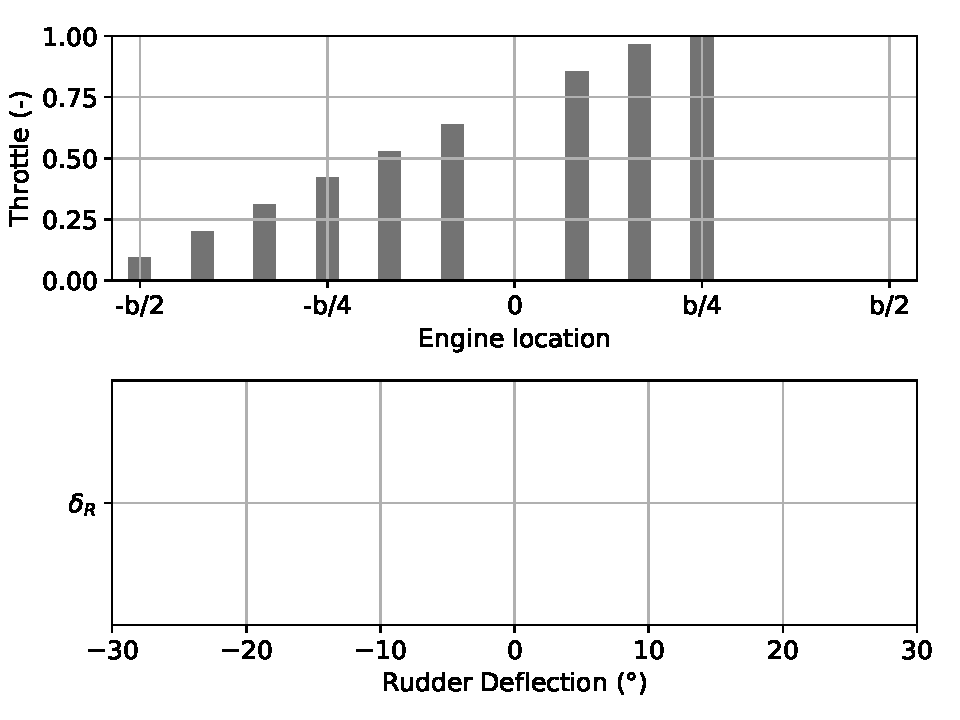
\includegraphics[width=0.95\textwidth]{DeflDEPoriginalfin07Eng15RudTrue}
		\caption{Throttle level and Rudder deflection at 60m/s and $\beta=0\degree$, ATR72 with 12 engines, three inoperatives, $S_v=0.7S_{v_0}$.}
		\label{fig:DeflDEPoriginalfin07_15Eng}
	\end{subfigure}
\end{figure}

%----- Study Case -----
%One original ATR72 at take off without failed engine next to the same ATR72 at Take off with SEF:
%	Shows that Vmc is found for take off,
%	Show that control is maintained at 1.3Vsr (=15° yaw toward inoperative engine)
%	shows that no equilibrium exists,
%	eventually show the degradation of equilibrium with reduced VT
%	Show the engine saturation at high speed

%Show the same ATR with distributed propulsion:
%	Show input histogramme with and without rudder
%	Show map without rudder and with small rudder
%	Show map with small fin and rudder
%
%At take off means :
%	3% slope for more than 4 engine condition, 
%	2.4 % for twin engine with landing gear retracted (CS.25.121)
%	Not necessarly full power but explore by going higher (in speed mostly)
%	0 altitude
%Maybe replace velocity scale by Vsr, 1.3Vsr etc... as defined by CS

% ATR at 21.5T Vapp=56m/s if it is 1.13Vsr then Vsr=49.55m/s, 1.3Vsr=64.4m/s
% Eventually look at the 20° turns requirement from the certif

%
%Determine 1.3V_{sr} for CS25.147 stating 15° yaw in the direction of the inoperative engine.
%STATE MINIMUM DRAG and 